\section{Przedstawienie dostępnych pułapek do zbudowania w grze Orcs must die!. Zofia Sosińska}\label{chap:omd}

Orcs must die! to strategiczna gra akcji stworzona i wydana przez studio Robot Entertainment. Akcja toczy się w krainie fantasy, w której największym zagrożeniem dla ludzkości są orkowie. W obronie świata przed tymi stworzeniami staje Zakon dowodzony przez Wojennych Magów. Wznieśli oni system fortec odgradzających ojczyznę orków od pozostałych ziem. Zadaniem gracza jest wcielenie się w jednego z  Wojennych Magów i mordowanie nadciągających grup orków za pomocą różnorodnych broni i mechanizmów, które może postawić.
W przejrzysty sposób zostało rozwiązane samo wyświetlenie dostępnych do zbudowania pułapek. Graczowi pokazują się wizerunki mechanizmów, które może postawić. Naciskając odpowiedni numer na klawiaturze, gracz wybiera, co chce zbudować. Po zatwierdzeniu lewym przyciskiem myszki, budynek pojawia się w zaznaczonym miejscu.

\begin{figure}[h!tbp]
    \centering
    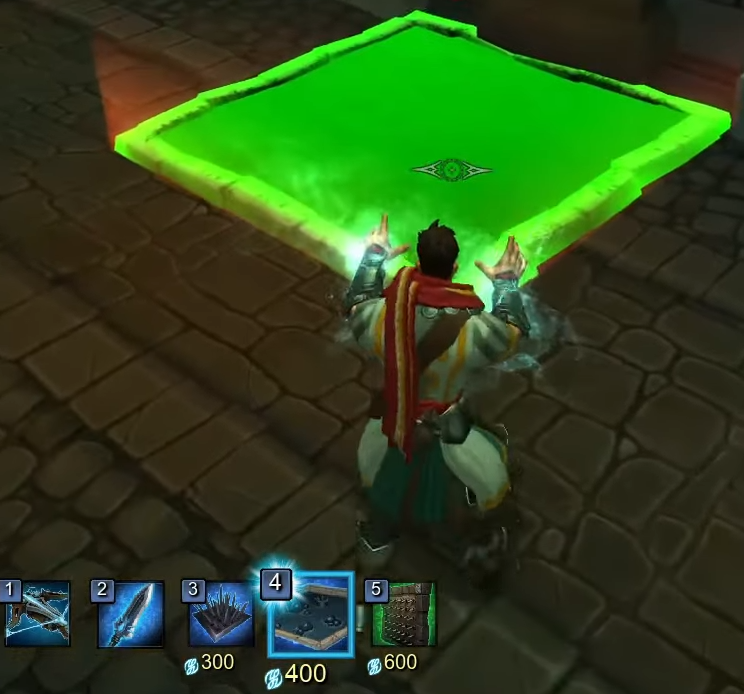
\includegraphics[width=0.9\textwidth]{images/ui/buoildingsOrcs.png}
    \caption{Wyświetlenie dostępnych pułapek w Orcs must die!}\label{fig:Orcs}
\end{figure}
